% SPDX-License-Identifier: Apache-2.0
\documentclass[11pt,letterpaper]{article}
\usepackage[margin=0.88in,headheight=16pt]{geometry}
\usepackage{fontspec}
\setmainfont{NimbusRoman-Regular.otf}[BoldFont=NimbusRoman-Bold.otf,ItalicFont=NimbusRoman-Italic.otf,BoldItalicFont=NimbusRoman-BoldItalic.otf]
\setsansfont{NimbusSans-Regular.otf}[BoldFont=NimbusSans-Bold.otf,ItalicFont=NimbusSans-Italic.otf,BoldItalicFont=NimbusSans-BoldItalic.otf]
\setmonofont[Scale=0.82]{DejaVu Sans Mono}
\usepackage{amsmath,amssymb,amsthm,mathtools}
\usepackage{microtype,graphicx,booktabs,tabularx,array,longtable}
\usepackage[table]{xcolor}
\usepackage{enumitem,fancyhdr,titlesec,caption,float,needspace}
\usepackage[most]{tcolorbox}
\usepackage{xurl,hyperref}
\definecolor{ink}{HTML}{102824}
\definecolor{teal}{HTML}{166D61}
\definecolor{amber}{HTML}{B96C2E}
\definecolor{paper}{HTML}{F5F3EC}
\definecolor{muted}{HTML}{52665F}
\hypersetup{colorlinks=true,linkcolor=teal,citecolor=teal,urlcolor=teal,
 pdftitle={AGI ALPHA FLYWHEEL: The Profitable Possibility Engine},
 pdfauthor={Vincent Boucher, President of MONTREAL.AI},
 pdfcreationdate={D:20261028},pdfmoddate={D:20261028},
 pdfsubject={An executed bounded exact-world campaign, adversarial enterprise economics, and successor challenge}}
\pagestyle{fancy}\fancyhf{}
\fancyhead[L]{\small\sffamily\color{muted}AGI ALPHA / TRANSFORMATIONAL INTELLIGENCE}
\fancyhead[R]{\small\sffamily\color{muted}28 OCTOBER 2026}
\fancyfoot[L]{\small\sffamily\color{muted}Executed research edition}
\fancyfoot[R]{\small\sffamily\thepage}
\renewcommand{\headrulewidth}{0.3pt}
\setlength{\parindent}{0pt}\setlength{\parskip}{0.48em}
\setlength{\emergencystretch}{2em}
\linespread{1.035}
\clubpenalty=10000
\widowpenalty=10000
\displaywidowpenalty=10000
\hyphenation{ALPHA}
\titleformat{\section}{\Large\sffamily\bfseries\color{ink}}{\thesection}{0.65em}{}
\titleformat{\subsection}{\large\sffamily\bfseries\color{teal}}{\thesubsection}{0.65em}{}
\titleformat{\subsubsection}{\normalsize\sffamily\bfseries\color{ink}}{\thesubsubsection}{0.65em}{}
\titlespacing*{\section}{0pt}{2.2ex plus 1ex}{0.7ex}
\titlespacing*{\subsection}{0pt}{1.4ex plus 0.6ex}{0.4ex}
\captionsetup{font=small,labelfont={bf,sf},skip=7pt}
\setlist{itemsep=2pt,topsep=3pt,leftmargin=1.5em}
\newcolumntype{Y}{>{\raggedright\arraybackslash}X}
\newcolumntype{P}[1]{>{\raggedright\arraybackslash}p{#1}}
\newcommand{\USD}[1]{US\$#1}
\newcommand{\status}[1]{{\sffamily\bfseries\color{teal}#1}}
\newtcolorbox{evidencebox}[1][]{colback=paper,colframe=teal,boxrule=0.6pt,arc=0pt,
 left=10pt,right=10pt,top=8pt,bottom=8pt,#1}
\newtheorem{proposition}{Proposition}
\newtheorem{definition}{Definition}
\newcommand{\F}{\mathcal F}
\newcommand{\E}{\mathbb E}
\newcommand{\N}{\mathbb N}
% Generated by build_report.py from frozen confirmation_v2 results.
\newcommand{\SmallCases}{128}
\newcommand{\Bijections}{504}
\newcommand{\PerformanceCases}{12}


\begin{document}
\begin{titlepage}
\color{ink}
{\sffamily\small\bfseries MONTREAL.AI\hfill TRANSFORMATIONAL INTELLIGENCE $\infty$\par}
\vspace{0.7in}
{\sffamily\fontsize{35}{38}\selectfont\bfseries AGI ALPHA\par FLYWHEEL\par}
\vspace{0.2in}
{\sffamily\fontsize{22}{26}\selectfont The Profitable\par Possibility Engine\par}
\vspace{0.25in}
{\Large Exact worlds, complete costs,\par and the test of productive inheritance\par}
\vspace{0.38in}
\begin{evidencebox}
\textbf{An executed campaign.}\quad A bounded computational instrument was built,
independently challenged, and used to construct fresh constrained ensembles.
Its enterprise and successor claims were then tested against stronger alternatives.
The evidence supports a useful research asset. It does not qualify a profitable
transformational flagship.
\end{evidencebox}
\vspace{0.25in}
\begin{tabularx}{\linewidth}{@{}YYY@{}}
\textcolor{teal}{\sffamily\bfseries CONSTRUCTION}&
\textcolor{teal}{\sffamily\bfseries ENTERPRISE}&
\textcolor{teal}{\sffamily\bfseries SUCCESSOR}\\[4pt]
Exact labeled ensembles, reusable instruments, and accepted outputs&
Stateful synthetic buyers, competition, complete costs, and cash&
Fresh concentration queries, transfer costs, and conventional controls
\end{tabularx}
\vfill
{\large\bfseries Vincent Boucher\par}
{\sffamily President of MONTREAL.AI\par Montréal, Québec, Canada\par}
\vspace{0.2in}
{\sffamily\small 28 October 2026 / Author review edition\par}
{\small Executed software evidence; explicitly simulated commerce; no customer receipts.\par}
\end{titlepage}

\section*{Abstract}
An enterprise that accumulates tools can still fail to expand what its successors can
profitably accomplish. We execute a campaign that tests the entire claim using a
specific digital production capability. Motivated by recent frontier releases and
continuing the AGI ALPHA program, we investigate exact construction of integer-table
ensembles with fixed margins, structural zeros, and individual capacity limits.
The resulting compiler groups columns only when their remaining constraints are
interchangeable, constructs a finite count graph, and delivers exact rank/unrank,
uniform samples, portable instruments, and concentration-conditioned ensembles.
The frozen confirmation contains \SmallCases{} tiny problems and \Bijections{}
exhaustive table bijections, plus \PerformanceCases{} larger synthetic requests.
All completed independent counts agree. An explicit failure on a published dataset
and successful conventional methods prevent a general invention claim.
A 24-month strategic economy separates contribution, complete project profit,
liquidity, customer custody, and real receipts. An initial policy and a revised
commitment-gated policy are evaluated on fresh scenarios; the frozen rule selects
no launch. Transferred successors are compared with fresh conventional construction,
specialized shortcuts, and equal conventional inheritance. The study contributes a
reproducible productive instrument, a linked falsification of overbroad commercial
and succession claims, and an operational distinction between possessing an asset
and expanding an economically attainable frontier. It establishes neither realized
profit nor an AI-specific discovery advantage.

\textbf{Keywords:} transformational intelligence; exact sampling; productive capability;
commercial simulation; working capital; successor evaluation; constraint compilation.

\begin{evidencebox}
\textbf{Reading the evidence.} ``Measured'' denotes executed computation in this
environment. ``Simulated'' denotes transactions between authored synthetic participants.
``Assumed'' denotes an unobserved commercial input. ``Unestablished'' means the required
evidence was not obtained. No synthetic buyer is an actual prospect, customer, or payment.
\end{evidencebox}

\setcounter{tocdepth}{1}
\begingroup
\small\setlength{\parskip}{0pt}
\makeatletter
\renewcommand{\l@section}[2]{\@dottedtocline{1}{0em}{1.8em}{#1}{#2}}
\makeatother
\tableofcontents
\endgroup
\clearpage

\section{A future worth constructing, and a first result that must earn it}

Consider an engineering or scientific workflow that needs entire families of possible
worlds, each satisfying hard aggregate requirements and known impossibilities.
Generating one plausible-looking example is easy. Manufacturing an exactly specified
ensemble, returning its cardinality, and conditioning it on a rare property can be
substantially harder. An example is a resource-allocation table whose row totals fix
available supplies, column totals fix requested loads, and zero cells forbid impossible
routes. Another is a scientific null ensemble with fixed margins and structural zeros.
The correct law depends on the scientific question; uniformity is a chosen specification,
not an automatic model of reality.

The longer-horizon possibility is a network of enterprises that constructs experimental
worlds and other productive instruments on demand. A first instrument enables questions
that its buyer could not previously afford to ask. A later instrument conditions,
combines, or extends those worlds. Accepted deliveries finance the construction of
new instruments. This is a meaningful future only if each causal step survives comparison
with established methods and complete costs.

The AGI ALPHA foundations distinguish a new formulation from better search inside a
fixed one, and a productive inheritance from a larger archive \cite{boucherTI,boucherEvolve}.
\emph{Invent the Economy} further separates technical capability from a voluntarily
accepted and financeable arrangement \cite{boucherEconomy}. The autonomous-enterprise
work makes reconstruction and capital requirements explicit \cite{boucherEnterprise}.
This campaign advances that program by exposing a real constructed artifact to a
stronger conventional comparator and a changing commercial environment.

\subsection{The six-link candidate}

\begin{tabularx}{\linewidth}{@{}P{0.20\linewidth}Y@{}}
\toprule
Link & What the campaign actually tests \\
\midrule
The constraint & Exact bounded ensembles can be difficult to enumerate or sample with a known law. This is not a universal impossibility claim.\\
The construction & A portable count-and-generation instrument for a declared finite problem.\\
The expansion & More feasible worlds and new concentration-conditioned outputs within measured budgets.\\
The commercial dependency & The delivered output is generated by the instrument; removing the generator removes the promised outcome.\\
The profit mechanism & An assumed fee for an accepted instrument or bundle must cover execution, review, acquisition, maintenance, and construction.\\
The successor option & A fresh exact concentration query using the inherited state graph, compared with fresh construction and equal conventional inheritance.\\
\bottomrule
\end{tabularx}

The first delivery directly exercises the proposed productive mechanism. It is not a
report recommending a generator, nor a dashboard checking someone else's output.
Nevertheless, a useful generator does not establish that the mechanism is new, that
buyers will pay, or that the retained artifact is economical to transfer.

\section{Why investigate now? A dated frontier with access boundaries}

The research window ends on 28 October 2026. The campaign emphasized the preceding
30 days, particularly the final week, and consulted original papers, author software,
and official release pages. Table~\ref{tab:frontier} separates a search signal from a
usable dependency. The accompanying source catalogue records URLs and retrieval dates.

\begin{table}[htbp]
\small
\begin{tabularx}{\linewidth}{@{}P{0.21\linewidth}P{0.12\linewidth}Y@{}}
\toprule
Development & Date & Implication and boundary \\
\midrule
GPT-6.1 Terra & 26 Oct & Official API/Work availability and posted token prices motivate cheaper artifact construction. Vendor benchmarks are not this campaign's measured costs or reliability \cite{terra,terraNotes}.\\
OpenAI scientific release & 26 Oct & Public mathematical and CS artifacts create new implementation leads. The authors describe the outputs as raw research data; practical algorithmic gains require separate work \cite{openaiScience}.\\
Genie 4 & 27 Oct & Research preview with restricted access and acknowledged simulation limitations. It is excluded as an essential dependency \cite{genie}.\\
SAT-fiber revision & 9 Oct & A current bounded-table competitor, with practical sampling-bias and runtime discussion; it supplies a prior-art challenge rather than novelty for this work \cite{satfiber}.\\
Haiku 5.5 / Mistral Large 4 & 7 / 6 Oct & Additional available or preview model options. Neither is an executed production dependency in the experiment \cite{haiku,mistral}.\\
\bottomrule
\end{tabularx}
\caption{Dated capability search. A release can motivate a construction without being experimentally shown to cause its advantage.}\label{tab:frontier}
\end{table}

The official Terra announcement lists \USD{1} per million input tokens,
\USD{0.05} per million cached input tokens, and \USD{5} per million output tokens
\cite{terra,terraNotes}. These are observed posted prices, not a reconstruction of
this session's invoice. The delivered deterministic sampler requires no model call
per table. Model-assisted design and review occurred during this campaign, but no
controlled old-model/new-model experiment or complete API usage ledger was available.
Consequently, the recent frontier is a motivating context, not an established causal
explanation of the numerical results.

\subsection{A consequential theorem that did not yield a practical product}

OpenAI's family 115 distinguishes exact uniform sampling without individual cell bounds
from randomized approximate counting with individual bounds \cite{openaiScope}.
Conflating them would create an unsupported claim of a general exact bounded sampler.
The source for the former prescribes an outer schedule
\[
T=d^{200}(k+b)^2,\qquad d\ge14.
\]
Even the factor $14^{200}$ is approximately $10^{229}$. This literal schedule is not a
finite production route here. The new manuscripts remain a research lead; their Lean
toolchain was not independently executed in this campaign \cite{openaiAlgorithm,openaiScience}.
The implemented dynamic program is a separate finite construction and does not inherit
those polynomial-time guarantees.

\section{Discovery, prior art, and the portfolio decision}

Three searches were combined. Future-backward search asked what means would make exact
conditional worlds cheap enough to use repeatedly. Frontier-forward search inspected
new constructive mathematical results. Need-inward search examined documented difficulties
in constrained scientific sampling and the free tools already addressing them.

\begin{table}[htbp]
\small
\begin{tabularx}{\linewidth}{@{}P{0.24\linewidth}YY@{}}
\toprule
Candidate & Decisive question & Disposition \\
\midrule
Literal new exact-sampling algorithm & Can its prescribed finite algorithm run at useful size? & Rejected for this execution envelope; no substitute was labeled as its implementation.\\
Bounded exact-world compiler & Can it deliver correct reusable ensembles and beat strong alternatives at complete cost? & Built and evaluated; useful construction, flagship qualification withheld.\\
Certified matrix-function production & Does a sharper theoretical constant improve an actual production operator against operator-specific conventional bounds? & Separately probed after the primary claims weakened; results retained in the alternative dossier.\\
General world-simulation service & Is essential model access and validated engineering fidelity available? & Excluded as a current dependency.\\
\bottomrule
\end{tabularx}
\caption{The portfolio retained alternatives and rejection reasons. Selection is not a novelty or valuation score.}
\end{table}

Miller and Harrison already developed exact counting, symmetry reduction, retained
count tables, and count-guided uniform sampling for fixed-margin matrices \cite{miller}.
Their actual EXACT v0.3 Python code is included as a licensed comparator, with two
recorded Python 3 compatibility changes \cite{exact}. Generic memoization, large
cardinalities, and reuse of a count graph therefore cannot establish novelty here.

Current SAT-fiber methods handle structural zeros and bounds, but use different finite-run
sampling guarantees \cite{satfiber}. Other established work treats approximate bounded
counting and exact sparse sampling \cite{cryan,sparse}. The campaign did not run every
external solver; it cannot claim superiority over that entire field. Its strongest executed
same-law comparator is an independently written conventional orbit dynamic program.
The authors' original algorithm is tested only on its supported binary domain.

SciPy's \texttt{random\_table} samples a fixed-margin conditional-independence law
\cite{scipy}. For nonnegative tables this generally weights a table by inverse cell
factorials. It is not the uniform-over-tables specification studied here. Its speed
does not satisfy that different contract, and its different output law is not a defect.
Similarly, population-synthesis software cannot be dismissed merely because it targets
realistic controls rather than our chosen ensemble \cite{population}.

\section{The constructed productive instrument}

\subsection{A finite contract}

For nonnegative integer row totals $r$, column totals $c$, and cell caps $U$, define
\begin{equation}
\F(r,c,U)=\{X\in\N^{m\times n}: X\mathbf1=r,\;X^\top\mathbf1=c,\;0\le X_{ij}\le U_{ij}\}.
\label{eq:fiber}
\end{equation}
A zero cap is a structural zero. The delivered law gives every labeled table in this
finite set probability $1/|\F|$. Invalid requests, empty sets, and exhausted construction
budgets receive different outcomes. A resource refusal is never reported as proof that
the fiber is empty.

The Python input boundary allows 1--16 rows, 1--96 columns, cell caps 0--16, equal total
mass no greater than 10,000, and explicit construction budgets. This is a syntactic
admission boundary, not a promise that every accepted shape compiles. The default
construction budget is 100,000 states, 1.5 million attempted transitions, and 30 seconds.
The browser publishes its smaller practical boundary separately. Exact integer arithmetic
is used for cardinalities and rank intervals.

Exactness concerns the integer count and the mapping from ranks to tables. The
law is uniform when supplied uniform integer ranks. Saved runs use a seeded
pseudorandom generator for repeatability; they do not establish infinite-sequence
independence or cryptographic unpredictability.

\subsection{The symmetry that is allowed}

At row depth $i$, a column's future signature is
\[
s_i(j)=(U_{ij},U_{i+1,j},\ldots,U_{m-1,j}).
\]
Columns are grouped only when both their remaining total and future signature agree.
For a group of $h$ such columns, let $a_v$ columns receive value $v$ in the current row.
The occupancy choice obeys $\sum_v a_v=h$ and has labeled multiplicity
\begin{equation}
M(a)=\frac{h!}{\prod_v a_v!}.
\label{eq:mult}
\end{equation}
All groups' assigned mass must equal the current row total. Their residual totals and
shortened signatures define the child state. The count recurrence is
\begin{equation}
C(q)=\sum_{e:q\rightarrow q'}M_eC(q'),\qquad C(q_{\rm terminal})=1
\label{eq:count}
\end{equation}
for a feasible terminal state. Impossible states contribute zero.

\begin{proposition}[Correctness of the finite construction]
If the count graph contains every feasible occupancy transition, the recurrence
\eqref{eq:count} counts each labeled table in \eqref{eq:fiber} exactly once. A uniform
integer rank in $\{0,\ldots,C(q_0)-1\}$ decoded through the weighted intervals yields
the uniform law on the fiber.
\end{proposition}
\begin{proof}
Two columns with identical future caps are interchangeable through a bijection of
their remaining cells. An occupancy decision partitions labeled row assignments
into disjoint groups of size \eqref{eq:mult}. Each assignment has exactly the child
completion count. Different row assignments or child completions produce different
tables, and every valid table has one of these assignments. Induction on the remaining
rows proves the count recurrence. Dividing the rank interval into blocks of size
$M_eC(q')$, then into a multiset-permutation rank and child rank, gives an invertible
enumeration. Uniform ranks therefore induce uniform labeled outputs.
\end{proof}

This is a correctness argument for an implemented specification using established
counting principles, not a new general counting theorem. The implementation can still
have bugs, which is why it is challenged with a different cell-level enumeration and
independent conventional code.

\subsection{A small counterexample with a large consequence}

For row and column totals $(1,1,1)$ and
\[
U=\begin{pmatrix}0&0&1\\1&1&0\\1&1&0\end{pmatrix},
\]
exactly two tables exist. A tempting implementation that sorts all residual column
totals together, while retaining these cap positions, returns zero. Columns with
different future restrictions are not interchangeable. The negative control preserves
this failure and prevents an apparently faster but invalid construction from being
promoted.

\subsection{The delivery contract and product experience}

A completed computational delivery contains the request, portable instrument, sampled
tables, acceptance receipt, source digest, and explicit law. The standalone bilingual
browser product performs real local construction and shows the resulting tables.
Its request, build, independent cell check, acceptance, and receipt stages are executable.
Its payment record is explicitly simulated; it contains no real checkout or transfer.

\begin{figure}[htbp]
\centering
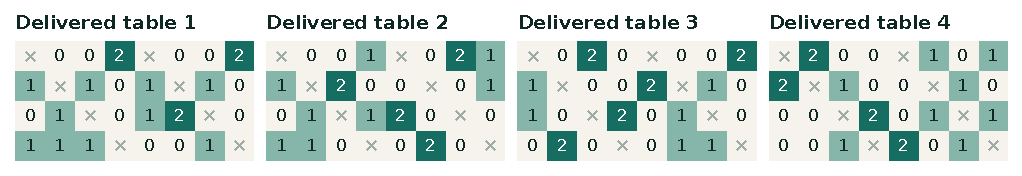
\includegraphics[width=\linewidth]{figures/instrument_worlds.pdf}
\caption{Four actual outputs from the separate 1,000-table example delivery.
Every row sums to four, every column to two, and each crossed cell is a structural
zero. The requested fiber contains 20,322 labeled tables. The portable instrument
and all 1,000 accepted outputs are included; this illustration is not an extra
held-out confirmation sample.}
\end{figure}

The separate output checker verifies integer cells, row totals, column totals, and
every cap directly. Tiny cases additionally establish full family equality and complete
rank/unrank bijections. This independently checks the generated outputs; it is not an
institutional audit of the whole software or the statistical suitability of the law.

\section{Frozen scientific evaluation and actual results}

\subsection{Protocol, correction, and provenance}

Development probes were kept separate from confirmation. The first scientific protocol
completed its tiny-instance stage, then aborted because the harness failed to record
a compiler resource refusal on the published finch case. A separate annotation-only
reference edit also arrived after that freeze. The original source bytes, protocol,
partial outputs, and failure log are preserved. They are not described as a completed
frozen campaign.

The corrected second protocol freezes source hashes, fresh seeds, case generators,
resource limits, comparators, and acceptance rules before execution. It records refusals
instead of aborting the comparison. No algorithmic change to the compiler was made
between these two protocols. The evaluator was not an independent institution and
the synthetic distributions were authored by the campaign; fresh seeds do not turn
them into representative industrial samples.

% SPDX-License-Identifier: Apache-2.0
% Generated by publication/build_science_figures.py; no experiments are run.
% Frozen inputs: results/confirmation_v2/{confirmation,performance,published_comparator}.json
% Post-confirmation inputs: alternatives/ordering/ordering_results.json
% Alternative inputs: alternatives/matrix_action/matrix_probe_{results,assessment}.json
% External sources: cite keys miller, exact, lorist, davidson, openaiMatrix.
\subsection{Exact agreement and accepted production}

The corrected confirmation completed \textbf{128 tiny instances}, including
\textbf{504 exhaustive table bijections} and \textbf{270 conditioned-output checks}.
Every tiny-instance count agreed with the independent enumerator. Enumerated feasible
tables were compared with the compiler's entire ranked family, including rank/unrank
inverses. These are finite exhaustive checks on the declared cases; they do not replace
the argument that multiplicity-weighted decoding samples the intended labeled law.

The larger campaign completed \textbf{12 synthetic requests} and delivered
\textbf{1,200 accepted tables}: 100 independently cell-checked outputs per request.
Construction took 0.0073--4.6444 seconds in the recorded executions.
The strongest independently written conventional counter completed 11 of
the 12 cases during confirmation, with matching counts in each. Its last case
timed out. The remaining count was corroborated only in the subsequent ordering
diagnostic described below; it is not retroactively counted as an independent result
of the frozen confirmation.

\begin{figure}[H]
\centering
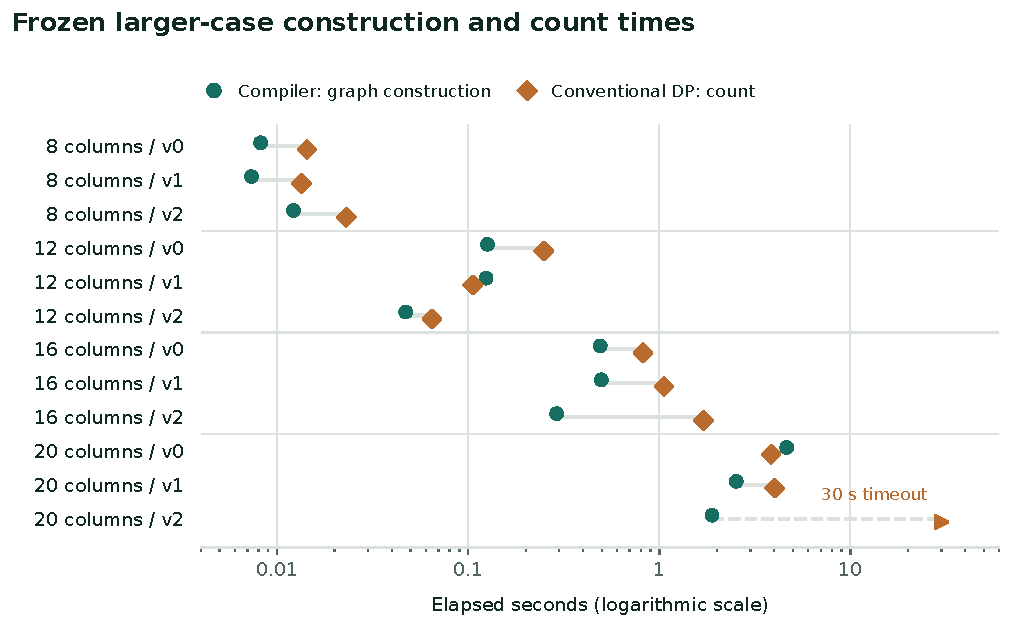
\includegraphics[width=\linewidth]{figures/scientific_performance.pdf}
\caption{All twelve larger cases from the corrected frozen campaign. Variants change
the margins and, for v2, add forbidden cells. Circles measure graph construction;
diamonds measure independent conventional counting. The right-pointing marker is a
30-second timeout, not a completed count. These are single executions, not repeated
performance estimates. Source: the frozen \texttt{performance.json} record.}
\label{fig:scientific-performance}
\end{figure}

\begin{table}[H]
\centering\small
\begin{tabular}{@{}rrrrr@{}}
\toprule
Columns & Exact labeled tables & Graph states & Compiler (s) & Conventional (s)\\
\midrule
8 & $20\,322$ & 106 & 0.0082 & 0.0143\\
12 & $14\,875\,620$ & 367 & 0.1262 & 0.2486\\
16 & $12\,763\,583\,010$ & 1,012 & 0.4913 & 0.8237\\
20 & $11\,973\,051\,233\,892$ & 2,354 & 4.6444 & 3.8548\\
\bottomrule
\end{tabular}
\caption{The four regular v0 controls, with four rows and column totals of two.
Both symmetry-aware implementations return the displayed counts. Large family size
is an output property; it does not by itself demonstrate algorithmic novelty.}
\label{tab:scientific-regular}
\end{table}

The simpler labeled-cell counter completed the three eight-column cases and reached
its state budget on the other nine. This comparison supports the usefulness of
column symmetry on these inputs. The independent orbit counter uses the same known
structural principle and is the more consequential conventional comparison.

\subsection{A published counterexample and a charged ordering repair}

The published $13\times17$ Darwin-finch binary-margin problem provides an external
check on the scope of the implementation. The authors' actual EXACT source, with
documented Python-3 compatibility edits, returned
\(67\,149\,106\,137\,567\,626\) in \textbf{0.40397 seconds}.
The new bounded compiler refused at its declared state/transition budget after
20.32 seconds. This is a successful conventional computation on a task
the constructed implementation did not complete. The published software's binary
scope is respected; unsupported arbitrary-cap tasks are not scored as incorrect
outputs~\cite{miller,exact}.

The final larger confirmation case initially appeared more favorable: the compiler
completed construction in 1.890 seconds while the conventional reference
timed out at 30 seconds. A separate post-confirmation challenge copied that reference
and changed only its row-order parameter. All 24 row permutations received the same
3.5-second execution budget. Eight finished, all returning
\(37\,877\,767\,916\); sixteen timed out. The best order took
\textbf{1.724 seconds}, and the ascending-row-sum permutation took 1.814 seconds.
Thus an ordinary ordering change reaches the compiler's recorded construction scale
on this observed case, without a new recurrence or pruning rule.

The entire diagnostic cost \textbf{75.177 seconds}, including unsuccessful
attempts. That search cost cannot be replaced by the winning attempt's runtime in a
first-use comparison. No general ordering policy was selected, and this adaptation
is not a fresh held-out result. The comparator returns a count; the compiler also
constructs a reusable transition graph. The small timing differences therefore do
not establish robust superiority in either direction.

\subsection{A second production route, executed and rejected}

The investigation also constructed an actual polynomial-action operator for
\(e^A v\), motivated by the sharp complete Crouzeix bound reported in OpenAI
family 325~\cite{openaiMatrix}. It executed 144 matrix/tolerance cases over
48 matrices: Jordan, symmetric diffusion, and two nonnormal convection-diffusion
families, at dimensions 16--128 and absolute tolerances $10^{-6}$, $10^{-10}$,
and $10^{-12}$. All produced vectors met their thresholds against a numerical
\texttt{expm} reference. Representative inputs, outputs, and reference vectors are
preserved, so this was a production probe rather than a certificate-only proposal.

The proposed theorem dependency fails a stronger prior-art check. The scalar
Crouzeix constant two needed by \(e^A v\) was already public in August 2026;
the newly complete matrix-valued scope is unused here~\cite{lorist}.
More decisively, this implementation encloses the numerical range in a disk.
The classical numerical-radius dilation and Okubo--Ando result already make that
disk a \emph{complete} 2-spectral set. Consequently the entire constant-two
polynomial program is also an existing conventional construction, with the same
degree, recurrence, and output~\cite{davidson}.

\begin{figure}[H]
\centering
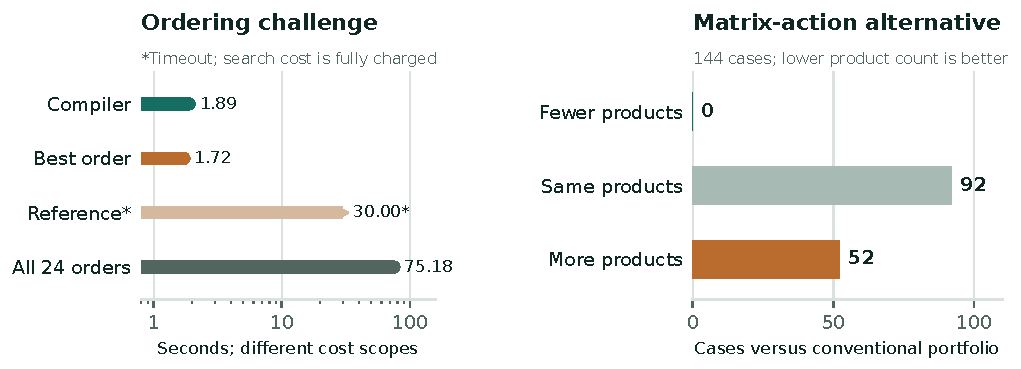
\includegraphics[width=\linewidth]{figures/scientific_challenges.pdf}
\caption{Two challenges after the frozen confirmation. Left: the ordering diagnostic
separates the winning conventional execution from the charged 24-order search;
the 30-second reference point is the original censored confirmation result.
Right: the executable matrix-action candidate uses fewer, equal, or more products
than a conventional portfolio containing the identical classical disk bound,
operator-norm bounds, normal-matrix bounds, and Jordan nilpotency. The portfolio
comparison is by degree, not a measured optimal portfolio runtime.}
\label{fig:scientific-challenges}
\end{figure}

Against the weaker general multiplier $1+\sqrt2$, substituting two saved one
matrix-vector product in 18 cases: 4,194 products became 4,176,
an aggregate reduction of 0.43\%. Against the stronger conventional
portfolio, the candidate had \textbf{0 lower-degree cases, 92 ties, and 52 higher-degree
cases}. These results do not qualify a new productive operator. The recorded error
bound controls analytical truncation only; ordinary floating-point evaluation and
a numerical reference do not provide total roundoff certification. This route was
therefore rejected as the next flagship rather than promoted on its tighter bound.

{\small\color{muted}Evidence files: the frozen confirmation directory; the
byte-preserved dossiers in \path{alternatives/ordering/} and
\path{alternatives/matrix_action/}. Figure generation reads those records and runs
no new scientific experiment.}


\subsection{What the comparison does and does not establish}

All completed same-law counts agree. In some bounded cases the new implementation is
faster than the independently written conventional implementation; in others it is
slower. Single-run timings depend on code organization, row order, hardware, and concurrent
load. They are not evidence of a new complexity class or a broadly superior method.
The simpler labeled-state comparator sometimes reaches its state limit while both
symmetry-aware methods complete. That establishes the value of the known structural
reduction in these cases, not a unique AGI ALPHA invention.

The published binary example provides a stronger warning. The authors' actual code
completes a case on which this bounded implementation refuses at its declared budget.
An astronomical count can coexist with an ordinary conventional solution. The result
prevents an appealing demonstration from becoming a false novelty claim.

\section{SUCCESSOR \texorpdfstring{$\Omega$}{Omega}: new questions and the cost of inheritance}

\subsection{A genuinely different query on the constructed family}

The predecessor is asked to construct and sample the fiber. The successor is asked
for its exact concentration distribution and samples conditioned on a fresh level of
\begin{equation}
K(X)=\sum_{i,j}\binom{X_{ij}}2.
\end{equation}
This statistic counts within-cell pairs and distinguishes concentrated allocations
from more dispersed ones. It is not a calibrated real-world risk measure.

Each retained edge receives its row's contribution $\delta_e$. The successor evaluates
the generating polynomial
\begin{equation}
G_q(z)=\sum_{e:q\rightarrow q'}M_ez^{\delta_e}G_{q'}(z),
\qquad G_{\rm terminal}(z)=1.
\label{eq:polynomial}
\end{equation}
The coefficient $[z^k]G_{q_0}$ is the exact number of tables with concentration $k$.
The same integer-interval construction then generates conditioned tables without
rejection. This is standard semiring evaluation applied to the delivered graph.

The statistic is invariant under the permitted column permutations. A statistic naming
a specific column need not be. Extending to such a query requires refining the state
or retaining the necessary labels; attaching an arbitrary label-sensitive statistic
to the quotient would be incorrect.

\subsection{Four comparisons, not one flattering benchmark}

The campaign measures warm graph evaluation; cold inheritance including decompression,
parsing, integrity and structural validation; a fresh conventional all-statistics
dynamic program; and a fresh target-specific conventional solver. A conventional
system receives the identical inherited asset as an additional control and matches
its outputs. Compilation and export costs remain separately visible.

For $K=0$, a particularly strong conventional simplification clips every cap to one.
It is an exact equivalent problem, not an approximation. Comparing against rejection
sampling alone would hide this shortcut. Expected rejection-draw calculations are
reported only as analytic illustrations, not as measured conventional performance.

\subsection{Measured successor results}
The two successor problems have 14 and 18 columns, distinct from the 8, 12, 16,
and 20-column performance problems. They follow the same synthetic construction
family; they do not establish transfer to a new industrial domain. Both exact
concentration distributions agree with the independently implemented conventional
semiring dynamic program.

\begin{table}[htbp]
\centering\small
\setlength{\tabcolsep}{4pt}
\begin{tabular}{@{}lrrrrr@{}}
\toprule
Problem & Fiber size & Warm & Cold & Fresh, all $K$ & Fresh, $K=0$\\
\midrule
$4\times 14$ & 418,474,536 & 0.0063 & 0.2831 & 0.2474 & 0.0035 \\
$4\times 18$ & 379,555,919,108 & 0.0830 & 2.2568 & 1.5193 & 0.0085 \\
\bottomrule
\end{tabular}
\caption{Executed successor count queries; times are local seconds. Warm evaluates
the retained graph. Cold adds read, parse, and validation. Fresh all-$K$ computes
the same complete distribution from the request. Fresh $K=0$ computes only that
target, using the binary-cap equivalence. The target column is a different,
narrower contract, not an all-statistics speed comparison.}
\label{tab:successor}
\end{table}

\begin{figure}[htbp]
\centering
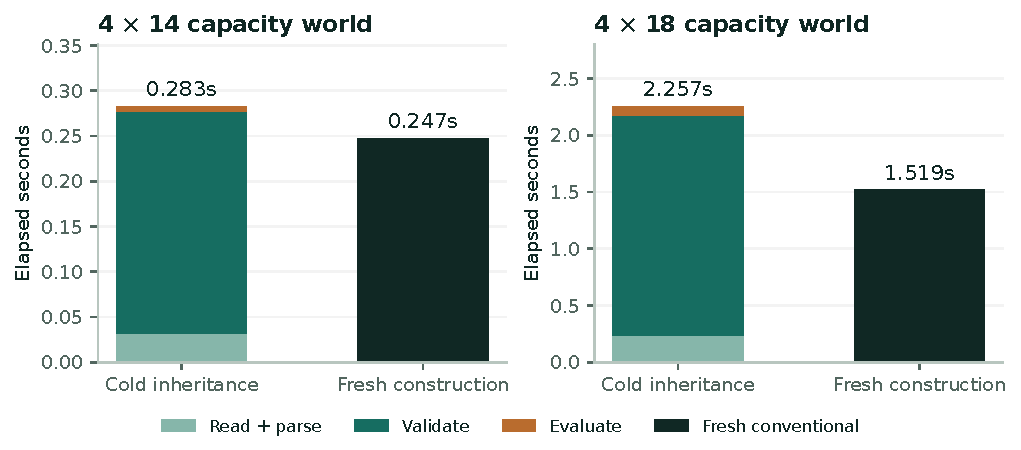
\includegraphics[width=\linewidth]{figures/successor_transfer.pdf}
\caption{Inheritance is useful in memory, but cold validation dominates these
transfers. Fresh conventional construction is faster for the same all-statistics
query on both held-out sizes. Predecessor construction and export are excluded
from these bars and reported separately below; adding them further increases
the full life-cycle cost of inheritance.}
\label{fig:successor}
\end{figure}

The 14-column asset has 504 states and 12,245 edges; the 18-column asset has
1,316 states and 76,943 edges. Their serialized JSON sizes are 1,339,844 and
8,512,360 bytes, compressed to 87,169 and 577,818 bytes. Predecessor construction
takes 0.1238 and 0.9237 seconds; export takes a further 0.1885 and 1.1112 seconds.
These costs are paid before the cold-query measurements. The complete construction,
export, and cold-query paths therefore take approximately 0.5954 and 4.2917 seconds.
No remote-network transfer or multi-year storage cost was measured.

\begin{table}[htbp]
\centering\small
\begin{tabular}{@{}lrrrr@{}}
\toprule
Problem & $K$ & Exact conditioned count & Generation seconds & Accepted tables\\
\midrule
$4\times 14$ & 0 & 94,968 & 0.0177 & 100 \\
$4\times 14$ & 1 & 996,336 & 0.0183 & 100 \\
$4\times 18$ & 0 & 5,444,610 & 0.0650 & 100 \\
$4\times 18$ & 1 & 78,007,280 & 0.0698 & 100 \\
\bottomrule
\end{tabular}
\caption{Fresh conditioned outputs generated from the inherited instrument.
Generation time is additional to obtaining the distribution and loading the asset.
Each of the 400 saved tables passes the original margins, caps, and requested
concentration check. These are computational acceptances, not customer acceptances.}
\end{table}

At 18 columns, only about $1.43\times10^{-5}$ of the uniform fiber has $K=0$.
That makes blind rejection unattractive, but the exact binary-cap simplification
computes its count in 0.0085 seconds. The separate target-specific comparator
measures counting, not generation of 100 outputs; no sample-generation speedup
over that comparator is asserted. The all-statistics comparison has the same
output contract on both sides.

The equal-inheritance control gives a conventional caller the same code and
artifact and obtains identical seeded conditioned outputs (20 at $K=1$ per
problem). This is an asset-availability control, not a second independent
implementation. It rejects exclusive ownership of the reuse benefit. The
independent full-distribution implementation supplies the separate numerical
correctness challenge.

\begin{evidencebox}
\textbf{Successor disposition.} Four hundred accepted conditioned worlds are
new outputs, and the instrument supplies a working productive inheritance.
The measured cold cost exceeds fresh conventional construction in both cases,
and conventional access to the same asset matches the result. Superior
transferred capability, an AI-specific advantage, and economically self-financing
succession are not established.
\end{evidencebox}


\subsection{Inheritance must carry its trust and maintenance costs}

The initial loader accepted an internally consistent digest without fully checking
edge semantics. The reviewer constructed a recomputed-digest alteration of the
concentration annotation. The repaired loader validates root states, occupancies,
child transformations, row depths, multiplicities, concentration increments, and terminal
mass. Without a separately retained trusted issuance digest, it reconstructs the
complete instrument to establish edge completeness. A self-supplied hash proves
neither correctness nor authenticity.

Six mutation cases and a resource-adversarial signature case are retained. The fast
inheritance experiment uses an issuance digest from the predecessor's accepted artifact.
Its measured transfer is a local read; remote transfer, access administration, and
long-term maintenance could add cost. Warm in-process speed is therefore an upper
view of reuse value, not the cost of constructing a new trusted successor elsewhere.

\section{A changing commercial economy}

\subsection{What is observed, what is assumed}

Published research documents useful applications of exact ensembles and practical
difficulties with approximate samplers. This supports a problem worth investigating.
It does not supply a purchase commitment. Free EXACT and SAT-based alternatives are
material competitive options. Adjacent posted prices include Mockaroo plans starting
at \USD{60} per year and GraphPad monthly plans of \USD{50} and \USD{75}
\cite{mockaroo,graphpad}. These price observations do not measure willingness to pay
for an exact-fiber instrument.

There are no actual prospects, accepted quotes, contracts, customer transactions, or
receipts in the campaign. All buyer valuations, budgets, demand rates, scope-fit
probabilities, acquisition responses, and retention behavior are authored assumptions.
The hypothetical market contains 240 synthetic organizations across scientific,
industrial validation, and synthetic-data segments. It is not a market-size estimate.
No credible billion-dollar reachable market is established.

\subsection{Participants and consequences}

Each buyer has a heterogeneous value, budget, DIY cost, scope fit, awareness, and
history. On a need event, the buyer compares the proposed service with DIY/free
software, a competitor, and abstention. It can refuse, negotiate, churn, reject a
delivery, or seek a subsequent refund. Failed deliveries affect future perceived
quality. Word of mouth and paid acquisition alter future awareness.

The competitor changes its price, quality, coverage, and distribution; visible market
share can trigger additional price cuts and imitation. Suppliers limit review capacity,
experience outages, and increase costs. The company has finite opening equity, a
bounded credit option, cash reserves, payables, accounts receivable, and delayed or
defaulted invoices. A cash-preserving shutdown can avoid insolvency while leaving a
large loss. Zero insolvency is not sustainable operation.

Common keyed random draws are used across policies to make comparable exogenous
conditions inspectable. The agents are explicit state machines, not independently
empirically trained people. Their separate incentives and state changes improve on
an independent-sales spreadsheet but do not validate the assumed market.

\subsection{Complete costs and the three economic tests}

The hypothetical launch charges 80 engineering hours at an assumed \USD{95} per hour,
\USD{800} of startup administration, and \USD{1,200} of equipment. Recurring maintenance,
administration, sales effort, hosting, accounting/insurance, periodic requalification,
and acquisition are charged. Per-attempt costs include review, support, retries,
processing fees, storage, failure handling, refunds, and bad debt. Equipment is
capitalized and depreciated; development is expensed. Financing and an explicitly
assumed tax treatment are separate. Actual historical campaign costs remain unmeasured
and are not falsely set to zero.

The economic histories simulate delivery attempts using assumed scope-fit,
acceptance, latency, and failure distributions. They do not execute the sampler
for each fictional order. An illustrative 0.6-second compute charge is anchored
to a local medium-size prototype, with an observed public serverless tariff
\cite{lambda}; it is not a hosting invoice or an industrial latency distribution.
Payment-processing assumptions use an observed published tariff \cite{stripe}.
Those narrow price anchors do not validate the assumed customer behavior.

For an accepted delivery, contribution is earned revenue after directly attributable
costs and reversals. Enterprise profit additionally deducts all recurring costs and
construction expenses. Cash requires the company to meet obligations at the time
they fall due. In the simulator, refundable customer advances increase cash and an
equal custody liability; they are unavailable for operating expenditure.

The exact cent ledger checks
\begin{equation}
\mathrm{cash}+\mathrm{receivables}+\mathrm{assets}
-\mathrm{custody}-\mathrm{payables}-\mathrm{debt}
=\mathrm{equity}+\mathrm{cumulative\ profit}.
\label{eq:balance}
\end{equation}
It also enforces $\mathrm{cash}-\mathrm{custody}\ge0$. A separate Decimal audit checks
the monthly CSV. Unchanged native AGI ALPHA arrangement code checks selected aggregate
cash bridges; that narrower check does not establish intramonth liquidity or demand.

\subsection{An initial failure followed by a controllable revision}

The first campaign evaluates self-service, qualified-instrument, subscription,
industrial-only, and stop policies. Training selects among complete-cost outcomes
using a frozen risk rule, then evaluates fresh worlds. The best active policy does
not qualify for launch.

The revision changes an action the enterprise controls: it seeks a bounded cohort
of conditional commitments before paying the full construction cost. Commitments
expire and can be withdrawn. The policy pays for a six-month search, retains the
same delivery and maintenance assumptions, and requires the expected cohort
contribution to cover startup, three months of fixed commitments, and a reserve.
It does not increase buyer willingness to pay to rescue a desired result. A policy
that never launches must still pay its search and closeout costs.

Both sources and configurations are frozen before their own confirmation runs.
The revised policy uses a new seed interval and is evaluated with the earlier active
policies. This is a preserved revision, not a retuned claim on the first test set.

% GENERATED from archived economic results by build_economic_figures.py.
% Actual customers and receipts remain zero; all monetary results below are simulated.

\subsection{Frozen results: the unit contributes, the enterprise loses}

The initial confirmation contains 3,584 worlds; the revised confirmation contains
7,168 worlds, with 256 worlds per policy--scenario cell. The original best active
training policy was the \USD{349} subscription. After the revision, the precommitted
rule still selects \textbf{stop}. The commitment gate is the least-loss spending
policy, but no spending policy qualifies as profitable.

In the fresh base worlds, the \USD{449} instrument produces mean revenue of
\USD{5,399.72} and mean total contribution of \USD{4,145.41}. Contribution
per net retained order averages \USD{339.84} across world-level ratios; this is a conditional modeled
commercial margin, not a measured market price. The enterprise delivers only
12.14 retained orders over 7.01 active months on average. Its recurring
operating result is \(-\)\USD{17,997.71}; including the launch expense, its
full-project result is \(-\)\USD{26,397.71}. Figure~\ref{fig:economic-bridge}
shows why a large per-order margin is insufficient.

\begin{figure}[htbp]
\centering
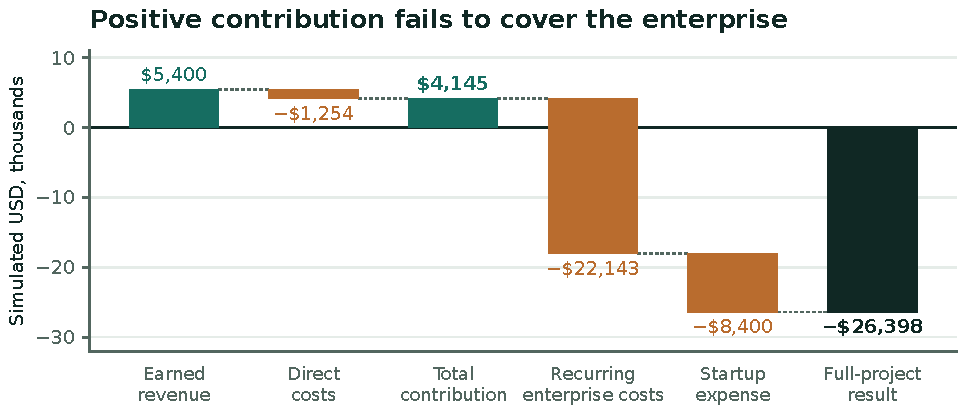
\includegraphics[width=\linewidth]{figures/economic_cost_bridge.pdf}
\caption{Mean simulated base-case cost bridge for the qualified \USD{449}
instrument, 256 worlds. Revenue is net of refunds. Direct costs include failed
attempts, retries, processing, support and bad debt. Recurring costs include acquisition and
\USD{1,200} equipment depreciation; the separate \USD{8,400} startup expense
therefore avoids counting equipment twice. Initial startup cash outlay is
\USD{9,600}. Figure labels are rounded; the prose and ledger retain exact cents.}
\label{fig:economic-bridge}
\end{figure}

The subscription has a higher mean number of retained orders (19.37), but
still loses \USD{26,521.09} over the full project. The instrument's simulated
acquisition cost, including allocated sales labor, averages \USD{557.68} per buyer,
against \USD{410.88} lifetime contribution within the observed \emph{simulated}
history. Neither model produces enough accepted demand to absorb the complete
enterprise cost. Every operating confirmation history loses money; none repays startup or
continues for the entire 24-month operating window.

\subsection{Stress outcomes and the meaning of survival}

\begin{table}[htbp]
\centering\small
\begin{tabularx}{\linewidth}{@{}Yrrr@{}}
\toprule
Scenario & \shortstack{Qualified\\\USD{449}} & \shortstack{Subscription\\\USD{349}} & \shortstack{Commitment gate\\\USD{449}} \\
\midrule
Base & $-26{,}397.71$ & $-26{,}521.09$ & $-3{,}050.00$ \\
Competitive pressure & $-26{,}468.83$ & $-26{,}484.97$ & $-3{,}050.00$ \\
Demand shortfall & $-26{,}431.52$ & $-26{,}569.31$ & $-3{,}050.00$ \\
Supplier disruption & $-26{,}449.16$ & $-26{,}508.49$ & $-3{,}050.00$ \\
Cost inflation & $-25{,}218.99$ & $-25{,}405.01$ & $-3{,}725.00$ \\
Late payments & $-25{,}264.48$ & $-26{,}521.09$ & $-3{,}050.00$ \\
Combined downside & $-27{,}280.16$ & $-26{,}825.40$ & $-3{,}522.50$ \\
\bottomrule
\end{tabularx}
\caption{Mean simulated full-project profit in USD after all stated costs and
the assumed tax treatment. Each cell contains 256 fresh worlds. The stop policy,
omitted from the table, preserves initial capital and earns zero. No table entry
is realized revenue, a buyer quote, or evidence of willingness to pay.}
\label{tab:economic-stress}
\end{table}

All spending policies lose in every reported world, including the gate's search
expense when it does not launch. Insolvency frequency is zero: the operating
policies shut down before exhausting their reserve, and the revised gate does not
launch. This is loss containment, not sustainable cash generation. Cost inflation
can cause a smaller total loss by forcing earlier closure and fewer deliveries;
it does not improve the business. Late payment leaves the prepaid subscription
unchanged, making clear that invoice timing is not its binding commercial defect.

The base instrument's tenth percentile of profit is \(-\)\USD{27,456.34};
its ninetieth percentile is \(-\)\USD{25,449.74}. These percentiles describe
variation inside the authored economy. They cannot quantify uncertainty about
whether the assumed customer population or preferences exist.

\subsection{The revision improves the decision without inventing customers}

At the frozen base costs, the launch condition requires 57 simultaneous qualifying
commitments. The revised search obtains a mean peak of 4.32 and a maximum of 11
across the 256 base worlds. It launches in \textbf{0/256} worlds, earns no revenue,
and spends \USD{2,850} on search plus \USD{200} on closeout. Its unconditional
project loss is therefore \USD{3,050}; profit conditional on launch is
\texttt{null}, because the conditioning event never occurs.

\begin{figure}[H]
\centering
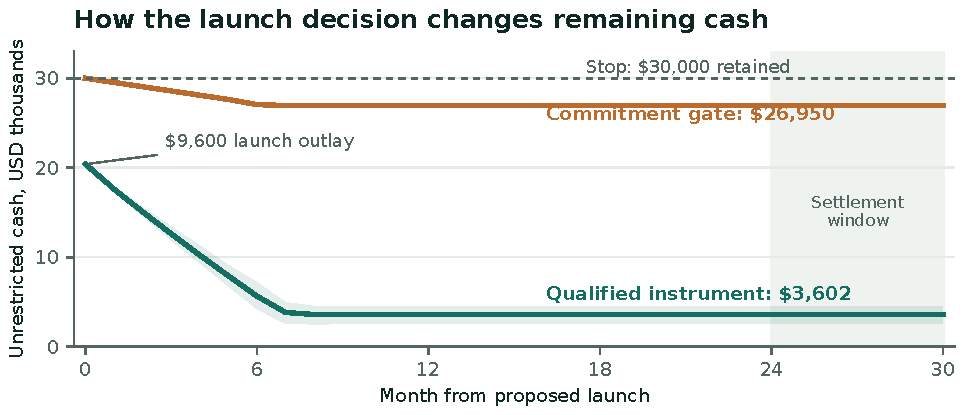
\includegraphics[width=\linewidth]{figures/economic_cash_paths.pdf}
\caption{Base-case unrestricted cash: means with pointwise tenth--ninetieth
percentile bands across the 256 synthetic worlds. The narrow gate path reflects
the same bounded search expenditure in every base world. The qualified offer
closes after a mean 7.01 active months; its terminal mean cash is
\USD{3,602.29}. The final six months settle outstanding obligations. No refundable
customer custody is spent on operations.}
\label{fig:economic-cash}
\end{figure}

The intervention succeeds at preserving more of the \USD{30,000} initial equity.
It does not establish a profitable commercial opening. The frozen rule's stop
decision is economically preferable to paying for a presale search that the
current assumptions predict will fail; neither decision satisfies Proof~II.

\subsection{Sensitivity and the limits of the economic evidence}

The static qualified-product calculation allocates construction, recurring costs,
requalification and closeout into about \USD{3,431.67} per month. At a nominal
\USD{449}, its expected contribution is \USD{345.81} per retained order, versus
the dynamic histories' mean of \USD{339.84}; the fixed-volume calculation omits
strategic price erosion and negotiated discounts. Approximately ten retained
orders per month would cover its burden, yielding only about \USD{634} pretax
over 24 months under constant-volume arithmetic. At \USD{349} the threshold
rises to fourteen orders, and at \USD{249}
to twenty-three. These are conditional thresholds, not jointly demonstrated
price--volume possibilities. Dynamic competition, acquisition, refunds and scope
refusal prevent the executed economy from reaching them.

A separate 40/80/160-hour replacement-construction sensitivity uses 32 new worlds
per policy and cost level. Both original operating policies continue to lose and
the commitment gate still refuses launch. Its control of timing helps preserve
capital without improving the unobserved willingness-to-pay premise. A large,
fully aware synthetic cohort was used only to exercise the simulator's launch
and positive-profit code branches; it is not an economic success scenario.

The corrected Decimal audit performs \textbf{3,512,320} monetary checks on the
revised confirmation and passes again under optimized Python. Twenty-one
archived participant traces replay exactly, and unchanged native AGI ALPHA code
agrees on 21 aggregate cash bridges. An original counter incorrectly included a
prior-month check in month zero; the original records and an explicit correction
are retained. Only that audit counter changed after confirmation, verified by an
AST comparison; no policy, outcome or money path changed. These checks establish
reproducible accounting within the model, not empirical demand or actual profit.



\subsection{What would have to change commercially}

A separate price--volume calculation reports a conditional break-even boundary. It
does not make every price and volume jointly attainable. The strategic simulator
retains price pressure, acquisition, scope rejection, and cash timing. The calculation
is useful for deciding which evidence is missing: sufficient accepted demand at a
contribution large enough to cover complete costs. The existing implementation's
cheap numerical execution alone does not meet that requirement.

The model includes no revenue from selling or licensing a successor transfer.
Maintenance and requalification are charged, but no unobserved monetary transfer
benefit is invented. Since complete historical research spending is unmeasured, even
a future positive launch simulation would not establish historical repayment.

\section{The opportunity frontier ledger and three proofs}

\begin{definition}[Budget-relative productive frontier]
For a method family $\mathcal M$, a resource allowance $B$, and an acceptance contract
$A$, let $\F_{\mathcal M}(B,A)$ be the tasks for which a method in $\mathcal M$ produces
an accepted result within $B$. A measured crossing is relative to those named methods,
that budget, and that contract; it is not a claim about all possible methods.
\end{definition}

The ledger distinguishes discovering an opportunity, implementing a capability,
crossing a declared computational budget, and creating a profitable activity. A
synthetic task newly accessible relative to labeled enumeration can already be
accessible to a conventional symmetry-aware method. A warm retained graph can enable
a fast query while the cost of transferring it destroys its complete advantage.

\begin{table}[htbp]
\small
\begin{tabularx}{\linewidth}{@{}P{0.20\linewidth}YY@{}}
\toprule
Required proof & Established evidence & Qualification \\
\midrule
I. Invention & Executable bounded production, independently checked exact outputs, explicit refusals & Useful instrument established; consequential novelty and superiority over strong prior art unestablished.\\
II. Enterprise & Contribution, profit, cash, adverse scenarios, and a revised policy executed & Simulated unit contribution can be positive; sustainable profitable enterprise not established; real receipts zero.\\
III. Expanding frontier & Fresh conditioned outputs, measured local transfer costs, direct conventional and equal-asset controls & Reuse works; superior transferred frontier and economic compounding not established.\\
\bottomrule
\end{tabularx}
\caption{The same instrument connects the three tests. Partial success is not promoted into the missing proofs.}
\end{table}

The linked Nova-Seed is therefore exploratory and not admitted. Its FusionPlan records
completed construction and experiments, failed claims, and the remaining evidence.
The opportunity ledger carries the exact comparison scope. No tokenization,
ownership representation, or new settlement system was needed to obtain these results.
Those mechanisms cannot compensate for a missing productive or commercial advantage.

\section{Limitations and intellectual contribution}

\textbf{External validity.} Most technical instances are generated software challenges.
The published finch example is real prior data, but it does not turn the synthetic
capacity worlds into industrial deployments. The chosen uniform law may be unsuitable
for a particular inference or operational simulation. The product provides no privacy
guarantee, causal guarantee, physical validation, or general statistical approval.

\textbf{Novelty and baseline coverage.} The main symmetry and count-guided sampling
ideas are established. The bounded implementation and product experience are new
code in this campaign; global algorithmic novelty is not proved. External SAT, C,
and specialized sparse implementations were not all run. Their unsupported cases
are not scored as failures. An unavailable dependency is a limitation of this run,
not evidence that a competitor cannot solve the problem.

\textbf{Autonomy.} The command-line delivery and browser computations run without a
person filling their intermediate tables. Research selection, code writing, and review
were performed by this AI-assisted campaign. No human/ordinary-model/expert-model
controlled study establishes operational alpha, retained alpha, or model-specific
superiority. Actual model usage costs and historical labor costs are unavailable.

\textbf{Commercial inference.} The simulator models stated hypotheses, not revealed
customer preferences. Monte Carlo precision only measures uncertainty under that
authored model. It cannot repair uncertainty about whether the market exists. The
correct decision under the current evidence is to withhold a paid-launch claim.

The principal contribution is an executed comparison of productive inheritance and
commercial feasibility in one causal chain. It shows how a capability can be correct,
useful, reusable, and still fail to qualify as a transformational enterprise. It also
identifies a concrete failure mode in successor evaluation: excluding parsing,
validation, transfer, and strong conventional reformulations can manufacture an
apparent frontier expansion. Preserving these costs changes the scientific result.

\section{Reproducibility and publication status}

The companion includes complete Python sources, the licensed original-code comparator,
frozen protocols and source snapshots, exact outputs, per-world economic results,
monthly ledgers, representative participant traces, source URLs, figures, the full
LaTeX source, and the standalone English/French product. The \texttt{README.md} gives
the commands and separates deterministic-output checks from variable wall timings.
The source manifest records SHA-256 digests. Digests bind bytes; they do not confer
approval or independent validation.

This study is additive to \path{MontrealAI/AGI-Alpha-Agent-v0}, based on commit
\nolinkurl{12770c22b4a9f90f2013bbfb64242f912ba5071e}. Existing routes, runtime authorities,
prior papers, frozen failures, and financial permissions are preserved. The relevant
native accounting code is reused for its narrow existing purpose. The study does
not assert a merge, a canonical deployment, or a new software release. Repository
qualification and publication status are recorded separately from local execution.

Scoped Ruff checks pass for the core scientific and economic sources. Strict Mypy
reports three typing diagnostics in the preserved kernel: two optional-integer
conversions in the private decoder and one repeated local annotation. The frozen
bytes and results remain unchanged; the draft does not claim a clean type check.
Full repository hooks, coverage, and hosted release qualification are not supplied
by this study's execution. The verification receipt records these boundaries.

\begin{evidencebox}
\textbf{Campaign disposition.} Retain the tested production instrument and its
negative evidence. Do not launch it as a qualified profitable flagship. The next
admissible advance must change the evidence: a substantive productive advantage,
an independently meaningful successor result, or accepted demand that covers complete
costs. None is supplied by a more ambitious name or a favorable unobserved sales rate.
\end{evidencebox}

\appendix
\section{Artifact map and exact reproduction boundaries}
All paths below are relative to
\path{studies/agi-alpha-profitable-possibility-v1/} in the pinned repository.
The standalone package preserves this study's directory layout.

\begin{longtable}{@{}P{0.37\linewidth}P{0.57\linewidth}@{}}
\toprule
Artifact & Purpose and boundary\\
\midrule
\endhead
\path{kernel.py}; \path{examples/} & Executable bounded count, rank, generation,
serialization, and successor operations. Core requires standard Python only.\\
\path{independent_reference.py}; \path{vendor/} & Independently written cell and
orbit comparators, original-author binary source, license, and provenance.\\
\path{configs/}; \path{archive/science_v1/} & Frozen protocols and source bytes
for the incomplete initial campaign. The completed v2 hashes bind current methods.\\
\path{results/confirmation_v2/} & Exact confirmation inputs, results, timings,
compressed inherited instruments, and 400 conditioned output tables.\\
\path{results/delivery_example/} & A separate complete 1,000-table delivery,
portable instrument, zero-revenue receipt, and independent cell acceptance record.\\
\path{results/browser_acceptance.json} & Chromium execution, responsive and
bilingual checks, downloads, finite-case bijections, and final copy-check chronology.\\
\path{economy.py}; \path{economics/} & Stateful simulated commerce; frozen
source/configuration, per-world summaries, monthly cent ledgers, decisions,
sensitivity, Decimal audits, and preserved errata.\\
\path{alternatives/} & Actual matrix-function outputs and prior-art challenge;
post-confirmation row-order diagnostic including the full charged search.\\
\path{product/index.html} & Standalone English/French local product; live
computation and exports, no external resources, real checkout, or hosting dependency.\\
\path{claim_register.json}; \path{opportunity_frontier.json} & Claim-to-evidence
map and budget-relative task ledger. Unestablished proofs remain unestablished.\\
\path{nova_seed.json}; \path{fusion_plan.json} & Exploratory candidate record
and completed execution record; neither grants launch or financial authority.\\
\path{research/}; \path{environment.json} & Verified source catalogue and
environment metadata. Timings are observations, not portable guarantees.\\
\path{publication/} & Complete LaTeX, generated section inputs, vector figures,
generation scripts, and compiled PDF.\\
\path{README.md}; \path{MANIFEST.sha256} & Full reproduction commands and
file digests. The manifest excludes itself and transient build caches.\\
\bottomrule
\end{longtable}

The original confirmation ledgers are retained without replacing their values.
The independent Decimal audit correction changes the performed-check counter,
not the economic histories. Reproduction must use a new output directory.
The original scientific protocol intentionally refuses execution against revised
method hashes; its archived source is supplied for inspection.

The core sampler, scientific harness, and economic simulation use the Python
standard library. Figure generation uses NumPy and Matplotlib; the alternative
matrix probe also uses SciPy. Browser automation uses Playwright and Chromium.
Opening the standalone HTML requires none of those build dependencies. The PDF
uses XeLaTeX with Nimbus Roman, Nimbus Sans, and DejaVu Sans Mono, with standard
TeX packages declared in the source. The environment record supplies the tested
versions without claiming that other versions are equivalent.


\section{Independent review, source credit, and research disclosure}

The independent computational review was performed by a separate agent with a
different implementation, before and after inspecting the kernel. It is distinct
from external peer review, formal proof of the Python interpreter, or an independent
customer acceptance process. The reviewer supplied the unsafe-sorting example,
original-author code, direct conventional successor shortcuts, and the loader mutation
challenge. The campaign corrected the observed loader failure before the completed
confirmation protocol.

The original EXACT comparator is copyright Jeffrey W. Miller and Matthew T. Harrison
under the accompanying BSD license. The adaptation records original and modified
hashes and the two syntax changes. New campaign code carries the repository's
Apache-2.0 notice. Public source manuscripts are cited as research inputs; their
theorems are not attributed to AGI ALPHA. Vincent Boucher is the requested author
and program lead; this edition was prepared through AI-assisted research, implementation,
and local execution, and is presented for author review.

\small
\begin{thebibliography}{99}
\bibitem{boucherTI} V. Boucher. \emph{Transformational Intelligence: Learning to Change the Game}. MONTREAL.AI, October 2026. \url{https://github.com/MontrealAI/AGI-Alpha-Agent-v0/blob/12770c22b4a9f90f2013bbfb64242f912ba5071e/docs/Transformational_Intelligence.tex}.
\bibitem{boucherEvolve} V. Boucher. \emph{Out-Evolve: Building the Means of Discovery and Production}. Revised manuscript, 20 October 2026. \url{https://github.com/MontrealAI/AGI-Alpha-Agent-v0/blob/12770c22b4a9f90f2013bbfb64242f912ba5071e/docs/Out_Evolve.pdf}.
\bibitem{boucherEconomy} V. Boucher. \emph{Invent the Economy: Transformational Intelligence for Creating Viable Markets}. October 2026. \url{https://github.com/MontrealAI/AGI-Alpha-Agent-v0/blob/12770c22b4a9f90f2013bbfb64242f912ba5071e/docs/Invent_the_Economy.tex}.
\bibitem{boucherEnterprise} V. Boucher. \emph{Autonomous Enterprises: Build the Means of Building}. Revised manuscript, 21 October 2026. \url{https://github.com/MontrealAI/AGI-Alpha-Agent-v0/blob/12770c22b4a9f90f2013bbfb64242f912ba5071e/docs/Autonomous_Enterprises.tex}.
\bibitem{terra} OpenAI. \emph{Introducing GPT-6.1 Terra}. 26 October 2026. \url{https://openai.com/index/introducing-gpt-6-1-terra/}.
\bibitem{terraNotes} OpenAI. \emph{Model Release Notes}. Entry 26 October 2026; retrieved 28 October. \url{https://help.openai.com/en/articles/9624314-model-release-notes}.
\bibitem{openaiScience} OpenAI. \emph{Working with academic communities to build scientific understanding}. 26 October 2026. \url{https://openai.com/index/building-scientific-understanding-with-academic-communities/}.
\bibitem{openaiScope} OpenAI. \emph{Sampling and counting contingency tables with arbitrary margins: formalization scope, family 115}. Retrieved 28 October 2026. \url{https://github.com/openai/math/blob/main/lean/docs/115.md}.
\bibitem{openaiAlgorithm} OpenAI. \emph{Exact Uniform Sampling of Contingency Tables with Arbitrary Margins}. Source section ``Sampling algorithms and exact correction'', September 2026 collection; retrieved 28 October. \url{https://github.com/openai/math/blob/main/preprints/Exact-Uniform-Sampling-of-Contingency-Tables-with-Arbitrary-Margins-September-24-2026/build/sections/algorithms.tex}.
\bibitem{genie} Google DeepMind. \emph{Genie 4: A new generation of world simulation}. 27 October 2026. \url{https://deepmind.google/blog/genie-4-a-new-generation-of-world-simulation/}.
\bibitem{miller} J. W. Miller and M. T. Harrison. Exact sampling and counting for fixed-margin matrices. \emph{Annals of Statistics} 41(3):1569--1592, 2013. DOI:10.1214/13-AOS1131. \url{https://jwmi.github.io/publications/Exact_matrix.pdf}.
\bibitem{exact} J. W. Miller and M. T. Harrison. \emph{EXACT v0.3 source distribution}. Retrieved 28 October 2026. \url{https://jwmi.github.io/software/exact_v0.3.zip}.
\bibitem{satfiber} P. Scharpfenecker and T. Windisch. SAT-sampling for statistical significance testing in sparse contingency tables. \emph{Statistics and Computing} 36, article 229, 2026; author revision 9 October 2026. DOI:10.1007/s11222-026-10985-8. \url{https://arxiv.org/abs/2511.05709v2}.
\bibitem{cryan} M. Cryan, M. Dyer, and D. Randall. Approximately Counting Integral Flows and Cell-Bounded Contingency Tables. \emph{SIAM Journal on Computing} 39(7):2683--2703, 2010. DOI:10.1137/060650544. \url{https://epubs.siam.org/doi/10.1137/060650544}.
\bibitem{sparse} A. Arman, P. Gao, and N. Wormald. \emph{Linear-time uniform generation of random sparse contingency tables with specified marginals}. Revised 15 June 2021. \url{https://arxiv.org/abs/2104.09413}.
\bibitem{scipy} SciPy developers. \emph{scipy.stats.random\_table}. Documentation retrieved 28 October 2026. \url{https://docs.scipy.org/doc/scipy/reference/generated/scipy.stats.random_table.html}.
\bibitem{population} ActivitySim contributors. \emph{PopulationSim documentation}. Retrieved 28 October 2026. \url{https://activitysim.github.io/populationsim/}.
\bibitem{mockaroo} Mockaroo. \emph{Plans and pricing}. Retrieved 28 October 2026. \url{https://mockaroo.com/}.
\bibitem{graphpad} GraphPad. \emph{Pricing}. Retrieved 28 October 2026. \url{https://www.graphpad.com/how-to-buy/}.
\bibitem{haiku} Anthropic. \emph{Claude Haiku 5.5}. 7 October 2026. \url{https://www.anthropic.com/claude-haiku-5-5}.
\bibitem{mistral} Mistral AI. \emph{Introducing Mistral Large 4}. 6 October 2026. \url{https://mistral.ai/news/mistral-large-4/}.
\bibitem{lorist} E. Lorist and F. L. Schwenninger. \emph{A solution to Crouzeix's conjecture}. arXiv:2608.03841v2, 17 August 2026. Preprint; not independently formally verified in this campaign. \url{https://arxiv.org/html/2608.03841v2}.
\bibitem{davidson} K. R. Davidson, V. I. Paulsen, and H. J. Woerdeman. \emph{Complete Spectral Sets and Numerical Range}. Author manuscript. \url{https://www.math.uwaterloo.ca/~krdavids/Preprints/DPWnum_range.pdf}.
\bibitem{openaiMatrix} OpenAI. \emph{The complete Crouzeix conjecture: formalization scope, family 325}. Retrieved 28 October 2026. \url{https://github.com/openai/math/blob/main/lean/docs/325.md}.
\bibitem{lambda} Amazon Web Services. \emph{AWS Lambda pricing}. Retrieved 28 October 2026. \url{https://aws.amazon.com/lambda/pricing/}.
\bibitem{stripe} Stripe. \emph{Pricing}. Retrieved 28 October 2026. \url{https://stripe.com/pricing}.
\end{thebibliography}
\end{document}
